\documentclass[tikz,border=8pt]{standalone}
\usepackage{tikz}
\usepackage{pgfplots}
\usepackage{amsmath,amssymb}
\usepackage[T1]{fontenc}
\usepackage{lmodern}
\usepackage{xcolor}
\usetikzlibrary{arrows.meta,positioning,shapes.geometric,fit,calc,backgrounds,matrix}
\pgfplotsset{compat=1.18}
\definecolor{ink}{HTML}{18202A}
\definecolor{blue}{HTML}{2563EB}
\definecolor{bluefill}{HTML}{EAF1FF}
\definecolor{green}{HTML}{14804A}
\definecolor{greenfill}{HTML}{E8F6EE}
\definecolor{amber}{HTML}{B56A00}
\definecolor{amberfill}{HTML}{FFF3D6}
\definecolor{red}{HTML}{B42318}
\definecolor{redfill}{HTML}{FDECEC}
\definecolor{gray}{HTML}{667085}
\definecolor{light}{HTML}{F4F6F8}
\definecolor{linegray}{HTML}{C7CDD4}
\tikzset{
  box/.style={draw=ink, rounded corners=3pt, very thick, fill=white, align=center, inner sep=7pt, font=\sffamily\small},
  bluebox/.style={box, fill=bluefill, draw=blue},
  greenbox/.style={box, fill=greenfill, draw=green},
  amberbox/.style={box, fill=amberfill, draw=amber},
  redbox/.style={box, fill=redfill, draw=red},
  ghost/.style={draw=linegray, rounded corners=3pt, thick, fill=light, align=center, inner sep=7pt, font=\sffamily\small},
  label/.style={font=\sffamily\footnotesize, text=gray, align=center},
  title/.style={font=\sffamily\bfseries\large, text=ink, align=center},
  arrow/.style={-{Latex[length=3mm,width=2mm]}, very thick, draw=ink},
  bluearrow/.style={-{Latex[length=3mm,width=2mm]}, very thick, draw=blue},
  redarrow/.style={-{Latex[length=3mm,width=2mm]}, very thick, draw=red},
  greenarrow/.style={-{Latex[length=3mm,width=2mm]}, very thick, draw=green}
}

\begin{document}
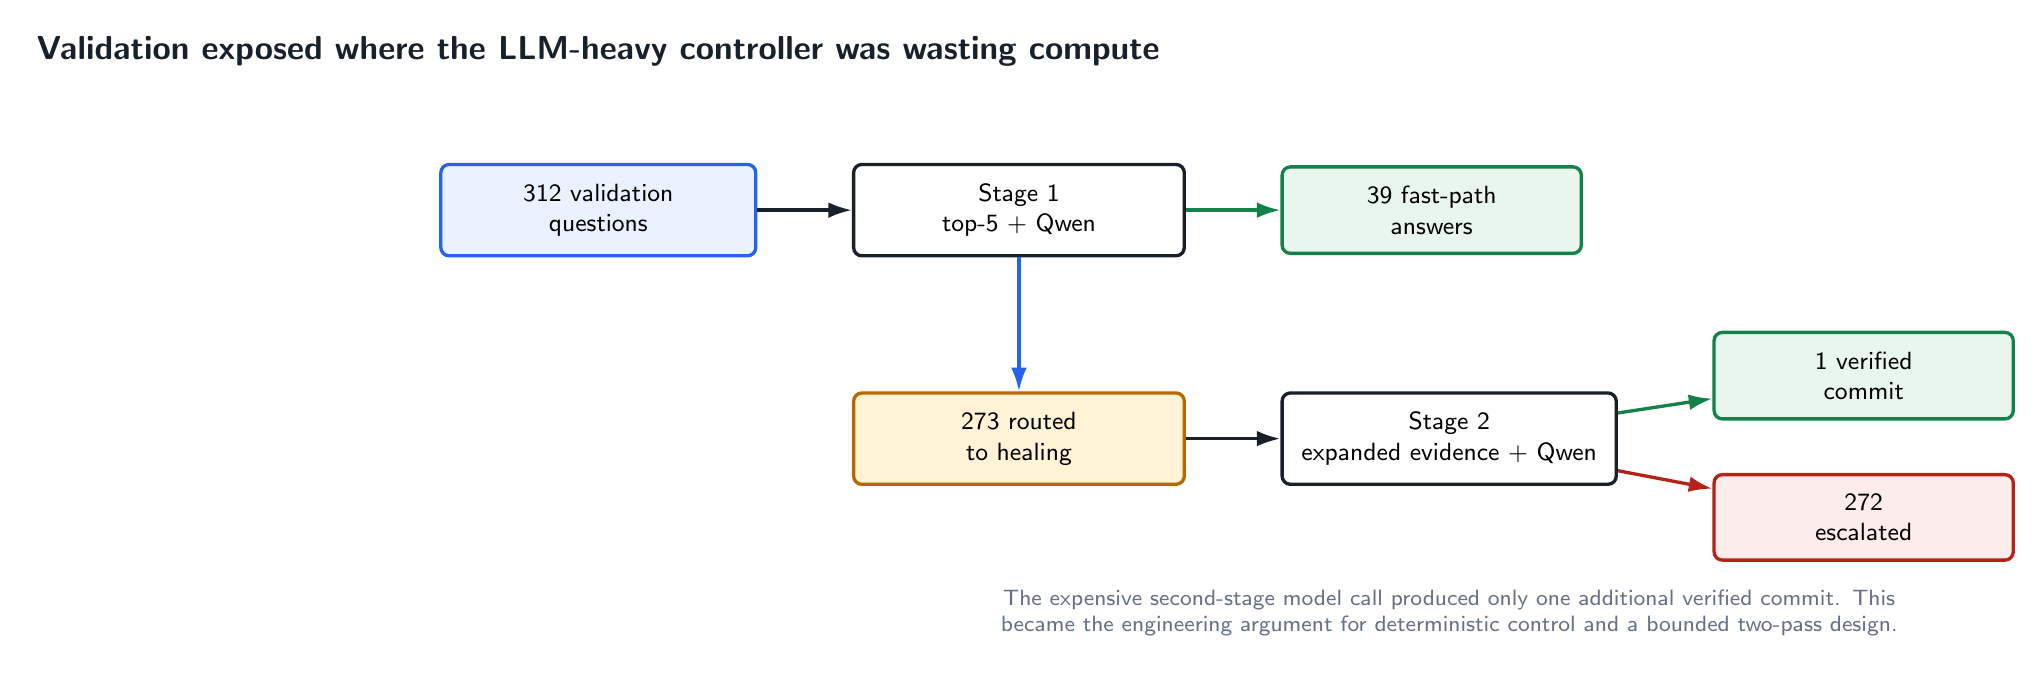
\begin{tikzpicture}[node distance=10mm and 12mm]
\node[title] (ttl) {Validation exposed where the LLM-heavy controller was wasting compute};
\node[bluebox, below=11mm of ttl, minimum width=40mm] (n) {312 validation\\questions};
\node[box, right=of n, minimum width=42mm] (s1) {Stage 1\\top-5 + Qwen};
\node[greenbox, right=of s1, minimum width=38mm] (fast) {39 fast-path\\answers};
\draw[arrow] (n)--(s1); \draw[greenarrow] (s1)--(fast);
\node[amberbox, below=17mm of s1, minimum width=42mm] (heal) {273 routed\\to healing};
\draw[bluearrow] (s1)--(heal);
\node[box, right=of heal, minimum width=42mm] (s2) {Stage 2\\expanded evidence + Qwen};
\draw[arrow] (heal)--(s2);
\node[greenbox, right=of s2, yshift=8mm, minimum width=38mm] (one) {1 verified\\commit};
\node[redbox, right=of s2, yshift=-10mm, minimum width=38mm] (esc) {272\\escalated};
\draw[greenarrow] (s2)--(one); \draw[redarrow] (s2)--(esc);
\node[label, below=12mm of s2, text width=135mm] {The expensive second-stage model call produced only one additional verified commit. This became the engineering argument for deterministic control and a bounded two-pass design.};
\end{tikzpicture}
\end{document}
